\documentclass[12pt,letterpaper]{article}

%%%%%%%%%%%%%%%%%%%%%%%%%%%%%%%%%%%%%%%%%%%%%%%%%%%%%%%%%%%%%%%%%%%%%%%%%%%%%%%
%% Preamble: load packages and set options
%%%%%%%%%%%%%%%%%%%%%%%%%%%%%%%%%%%%%%%%%%%%%%%%%%%%%%%%%%%%%%%%%%%%%%%%%%%%%%%

%%% AMS Math
\usepackage{amsmath}

%%% Bold math definitions
\usepackage{bm}

%%% graphics import support
\usepackage{graphicx}

%%% Misc. Packages
\usepackage{setspace}
\usepackage{color}
\usepackage{xspace}

\usepackage{achemso}

%%% Layout:
\usepackage[letterpaper,ignoreall,top=2.65cm,bottom=2.7cm,%
left=2.65cm,right=2.65cm,foot=1cm,head=1.5cm]{geometry}

%%%%%%%%%%%%%%%%%%%%%%%%%%%%%%%%%%%%%%%%%%%%%%%%%%%%%%%%%%%%%
%% Macro definitions
%%%%%%%%%%%%%%%%%%%%%%%%%%%%%%%%%%%%%%%%%%%%%%%%%%%%%%%%%%%%%
\newcommand{\transpose}{T}
\renewcommand{\vec}[1]{\ensuremath{\bm{#1}}\xspace}
\newcommand{\mat}[1]{\ensuremath{\bm{#1}}\xspace}
\newcommand{\ten}[1]{\ensuremath{\bm{#1}}\xspace}
\newcommand{\class}[1]{\textit{#1}\xspace}

\newcommand{\panache}{\textit{PANACHE}\xspace}
\newcommand{\Qso}{\ten{Q_{so}}}
\newcommand{\Qmo}{\ten{Q_{mo}}}
\newcommand{\Qoo}{\ten{Q_{oo}}}
\newcommand{\Qov}{\ten{Q_{ov}}}
\newcommand{\Qvv}{\ten{Q_{vv}}}

\newcommand{\edit}[1]{\textbf{\textcolor{red}{*** #1 ***}}\xspace}



%%%%%%%%%%%%%%%%%%%%%%%%%%%%%%%%%%%%%%%%%%%%%%%%%%%%%%%%%%%%%%%%%%%%%%%%%%%%%%%
%% Begin of Document
%%%%%%%%%%%%%%%%%%%%%%%%%%%%%%%%%%%%%%%%%%%%%%%%%%%%%%%%%%%%%%%%%%%%%%%%%%%%%%%

\begin{document}

\begin{center}
\large\textbf{\panache: A Modular Approach to Approximate Two-Electron Repulsion Integrals}
%
\vspace*{2ex}

\normalfont
\normalsize
%
Benjamin P.\ Pritchard, T.\ Daniel Crawford\\
{Department of Chemistry, Virginia Tech, Blacksburg, Virginia 24061, U.S.A.}\\
\vspace{2ex}
Robert M.\ Parrish, C.\ David Sherrill\\
{Center for Computational Molecular Science and Technology \\
School of Chemistry and Biochemistry, Georgia Institute of Technology, Atlanta, Georgia 30332, U.S.A.}\\
\vspace{2ex}
Andrew C.\ Simmonett \\
{Laboratory of Computational Biology, National Heart, Lung, and Blood Institute\\
National Institutes of Health, Rockville, Maryland 20892, U.S.A.}\\
\vspace{2ex}
Justin M\ Turney\\
{Center for Computational Quantum Chemistry, Department of Chemistry \\
University of Georgia, Athens, Georgia 30602, U.S.A.} \\

\date{\today}
\end{center}

%\textbf{\textcolor{blue}{LAST UPDATE: 2013-08-01}}
%%%%%%%%%%%%%%%%%%%%%%%%%%%%%%%%%%%%%%%%%%%%%%%%%%%%%%%%%%%%%%%%%%%%%%%%%%%%%%%

\doublespacing


\begin{center}
\textbf{Abstract}
\end{center}

The calculation of electron repulsion integrals (ERIs) over nucleus-centered
Gaussian-type functions is often among the most computationally intensive
tasks of quantum chemical models.  The memory required to store these
integrals --- ca.\ ${\cal O}(N^4)$, where $N$ is the number of basis functions
--- is often beyond the capacity of the computing hardware, thus necessitating
either repeated retrieval from slow, disk-based storage or ``on-the-fly''
recalculation.  A number of approximate ERI methods attempt to overcome this
bottleneck by decomposing the full integral matrix into products of tensors of
reduced rank [e.g., ${\cal O}(N^3)$], which either fit in memory or, at the
very least, significantly reduce the quantity of data to be transferred from
external storage.  However, the robust implementation of these methods
requires considerable software infrastructure, such as the ability to compute
ERIs with varying basis sets on different centers and out-of-core,
integral-direct decomposition algorithms, among others.  In this work, two of
the most widely-used ERI approximations --- density-fitting and Cholesky
decomposition --- have been implemented in a C++ library called the ``Parallel
Numerical Approximations in Chemistry Engine'' or \panache. The library is
designed to be modular and portable, and to support interfaces in multiple
programming languages.

\clearpage
%%%%%%%%%%%%%%%%%%%%%%%%%%%%%%%%%%%%%%%%%%%%%%%%%%%%%%%%%%%%%%%%%%%%%%%%%%%%%%%


\section{Introduction}
\label{sec:intro} 

Among the most computationally expensive and time-consuming steps in many
quantum chemical methods is the generation and manipulation of four-center
two-electron repulsion integrals (ERIs),
\begin{equation}
(\mu \nu | \rho \sigma) = \int \int \chi_\mu(\vec{r}_1) \chi_\nu(\vec{r}_1)
\frac{1}{r_{12}} \chi_\rho(\vec{r}_2) \chi_\sigma(\vec{r}_2)
d\vec{r}_1 d\vec{r}_2,
\end{equation}
where $\vec{r}_1$ and $\vec{r}_2$ are the spatial coordinates of electrons one
and two, respectively, and the $\chi_\mu$ are (typically) nucleus-centered
contracted Gaussian-type orbitals.  The calculation and storage of such ERIs
scales poorly [formally as ${\cal O}(N^4)$ with respect to the number of basis
functions, $N$], thus requiring either retrieval of the integrals from disk
(which is often very slow) or their on-demand recomputation (which can be
inefficient, depending on the application).  Alternatively, the ERI matrix,
which is a four-index tensor, may be decomposed into a product of three-index
tensors, {\em viz.},
\begin{equation}
(\mu \nu | \rho \sigma) = \sum_{Q} B_{\mu \nu}^Q B_{\rho \sigma}^Q,
\end{equation}

where the specific definition of the tensor, $B$, and the associated auxiliary
index, $Q$, depends on the choice of decomposition method. If the resulting
implementation yields a small enough dimension of $Q$, such decompositions can
significantly reduce the storage requirements as compared to the full-rank
ERIs, as the smaller tensors may either be retained completely in memory or
retrieved from external disk much more efficiently.  This reduction, in turn,
can substantially increase the speed of a number of key algorithmic steps in
electronic structure methods.  For example, the transformation of the
integrals from the atomic orbital (AO) to the molecular orbital (MO) basis
nominally scales as ${\cal O}(N^5)$, but this is reduced to ${\cal O}(N^3 Q)$

, the evaluation of the energy in second-order many-body perturbation theory, or the calculation of the coupled
cluster ground- or excited-state wave functions, among others.

  is also improved, a fact exploited in a number of
reduced-scaling many-body methods, such as...

Furthermore, the mathematical expressions involving the four-index tensors can
often be rewritten in terms of their lower-rank counterparts, potentially
reducing the scaling of expressions in, for example, second-order perturbation
theory or coupled cluster theory calculations.\cite{Werner:2003a} [Need lots
more references here.]


Two of the most popular techniques to approximate these tensors are density
fitting (also referred to as ``resolution of the identity'') and Cholesky
decomposition [need original references here], and these have been implemented
in a number of program packages.  [PSI4, Turbomole, Molcas, Molpro and others]




such as Gaussian\cite{Gaussian09}, Psi4\cite{Turney:2012a}, MPQC, and
others. 


Despite the overall gain in efficiency, implementing density fitting
or Cholesky decomposition can be tedious and time consuming, with the
feeling of 'reinventing the wheel'. In addition, retrofitting existing
code can be difficult as the code dealing with integrals is often among
the oldest and most heavily-optimized, and therefore least understood,
parts of computational chemistry software.

The motivation for \panache is to create a standalone library that
allows for the implementation of these approximate integral techniques
in new or existing code with minimal effort, freeing the programmer to
concentrate on other, more interesting parts of their code. It also aims
to demonstrate the power and flexibility of modular, object-oriented
design principles in the computational physical sciences.

\panache is based on code originally extracted from the
Psi4\cite{Turney:2012a} package, and heavily modified for efficiency
and to provide it with an interface usable from other software packages.


\subsection{Theory}
\label{sec:theory}

What follows is a brief outline of density fitting and Cholesky decomposition.
For a more detailed derivation and analysis, we refer the reader to the
relevant literature.

In density fitting,\cite{Werner:2003a,Dunlap:1977a,Dunlap:1979a,Whitten:1973a} a four-index ERI tensor can be approximated
using an auxiliary basis. Starting with the statement of the ERI
in terms of the repulsion between two electron densities
%
\begin{equation}
(\mu \nu | \lambda \sigma) = \int \int \rho_{\mu \nu}(\vec{r}_1) \frac{1}{r_{12}} \rho_{\lambda \sigma}(\vec{r}_2) d\vec{r}_1 d\vec{r}_2
\end{equation}
%
where $\mu$,$\nu$,$\lambda$, and $\sigma$ are genera atomic orbital indices.
The density $\rho_{\mu\nu}$ can be approximated using the auxiliary basis $\chi_Q$
and fitting coefficients $d_Q^{\mu\nu}$
%
\begin{align}
\tilde{\rho}_{\mu\nu}(\vec{r}) &= \sum_Q^{N}d_Q^{\mu\nu} \chi_Q(\vec{r}) \\
                           &= \sum_Q^{N}d_Q^{\mu\nu} ( Q |
\end{align}
%
where $N$ represents the number of basis functions in the fitting basis.
Commonly, these fitting coefficients are taken to be in the form\cite{Dunlap:1977a,Dunlap:1979a}
%
\begin{gather}
d_Q^{\mu\nu} = \sum_P (\mu\nu | P)[\mat{J}^{-1}]_{PQ} \\
J_{PQ} = \int \int \chi_P(\vec{r}_1) \frac{1}{r_{12}} \chi_Q(\vec{r_2}) d\vec{r}_q d\vec{r}_2 \label{eqn:metric}
\end{gather}
%
That is, the metric $\mat{J}$ can be obtained from two-center electron repulsion integrals
of the auxiliary basis.

Therefore, the full four-index ERI tensor can be written as a contraction involving
the metric (matrix) $\mat{J}$ and a three-index tensor
%
\begin{align}
(\mu\nu|\lambda\sigma) &= \sum_P^{N}d_Q^{\mu\nu} (Q | \lambda\sigma) \\
        &= (\mu\nu | P) [\mat{J}^{-1}] (Q | \lambda\sigma) \label{eqn:df-final}
\end{align}
%
where $(\mu\nu | P)$ and $(Q | \lambda\sigma)$ are formed from three-center electron
repulsion integrals involving the primary and auxiliary basis sets.

One particularly useful form of Eq.~\ref{eqn:df-final}
involves replacing $\mat{J}^{-1}$ with the product
$\mat{J}^{-\frac{1}{2}}\mat{J}^{-\frac{1}{2}}$ and simplifying

\begin{align}
( \mu\nu | \lambda\sigma ) &= (\mu\nu | P) [\mat{J}^{-\frac{1}{2}}]_{PQ} [\mat{J}^{-\frac{1}{2}}]_{QR} (R | \lambda\sigma) \\
              &= \sum_{Q}  B_{ab}^Q B_{cd}^Q
\label{eqn:df-simple}
\end{align}
%
where, keeping in mind the permutational symmetry of the three-index integrals
and the fact that $P$, $Q$, and $R$ are only summation indices
% 
\begin{equation}
B_{ab}^Q = \sum_P^N ( \mu\nu | Q ) [\mat{J}^{-\frac{1}{2}}]_{PQ} 
\label{eqn:df-simpleB}
\end{equation}
%
The advantage of such a form is the elimination of the need for storing the
metric separately. In addition, this allows for on-the-fly contraction
of $( \mu\nu | Q )$ with $\mat{J}^{-\frac{1}{2}}$ as it is generated.

In practice, the auxiliary basis is much larger than the primary basis
set, however in most cases the storage required for the three-index tensor
is much less than its four-index counterpart.  The $B_{pq}^Q$ tensor
(labeled \Qso within \panache the code) can also be transformed via the
MO coefficient matrix (or blocks thereof) to form \Qmo, \Qoo, \Qov, and
\Qvv for MO, occupied-occupied, occupied-virtual, and virtual-virtual
blocks, respectively. This transformation now scales $O(N_\mathrm{aux} N^2)$, rather
than a $O(N^4)$ transformation on the four-index ERI tensor.


In Cholesky decomposition,\cite{Roeggen:2008a,Beebe:1977a} the two-electron tensor (written as a matrix
with rows and columns corresponding to composite indices $a=(\mu\nu)$
and $b=(\lambda\sigma)$, respectively) can be written as a product of a lower
triangular matrix $\mat{L}$ and its transpose
%
\begin{equation}
(a | b) = \mat{V} = \mat{L}\cdot\mat{L}^{\transpose}
\end{equation}
%
where elements of $\mat{L}$ are determined by
%
\begin{align}
L_{ii} &= \left( V_{ii} - \sum_{k=1}^{i-1} L_{ik}^2 \right)^{\frac{1}{2}} \\
L_{ij} &= \frac{1}{L_{jj}} \left( V_{ij} - \sum_{k=1}^{j-1} L_{ik}L_{jk} \right), \qquad (j+1) \leq i \leq M
\end{align}
%
where $M$ represents the index of the last for of $\mat{V}$.
The generated $\mat{L}$ matrix is analogous to a three-index tensor,
similar to $B$ from density fitting, with $M$ rows and with columns corresponding
to the AOs of the basis set.
If the indicies of $\mat{L}$ are ordered where
%
\begin{equation}
L_{ii}^2 \geq V_{nn} - \sum_{k=1}^{i-1} L_{nk}^2, \qquad (j+1) \leq n \leq M
\end{equation}
%
The iterations may be stopped if $L_{ii}^2 \leq \delta$ where $delta$ represents
the desired accuracy. In this way, the number of rows of $\mat{L}$ are less than
$M$.

Since $\mat{L}$ is analogous to the three-index tensor from density fitting, 
it may be manipulated in an identical manner, including transformations to
the MO basis.


\section{Description and Features}
\label{sec:description}

\panache is written in C++11, with interfaces for use from C and Fortran
code. It is made to be portable -- it utilizes the CMake\cite{CMake} build system and
is relatively self-contained with few external dependencies.  The library
enforces strict separation of interface and implementation, thereby making
it modular and extensible. For example, it is relatively easy to add
new storage classes or different integral backends. Both density
fitting and Cholesky decomposition share nearly identical interfaces,
allowing easy adoption of either or both methods in new or existing code.


\begin{figure}
\centering
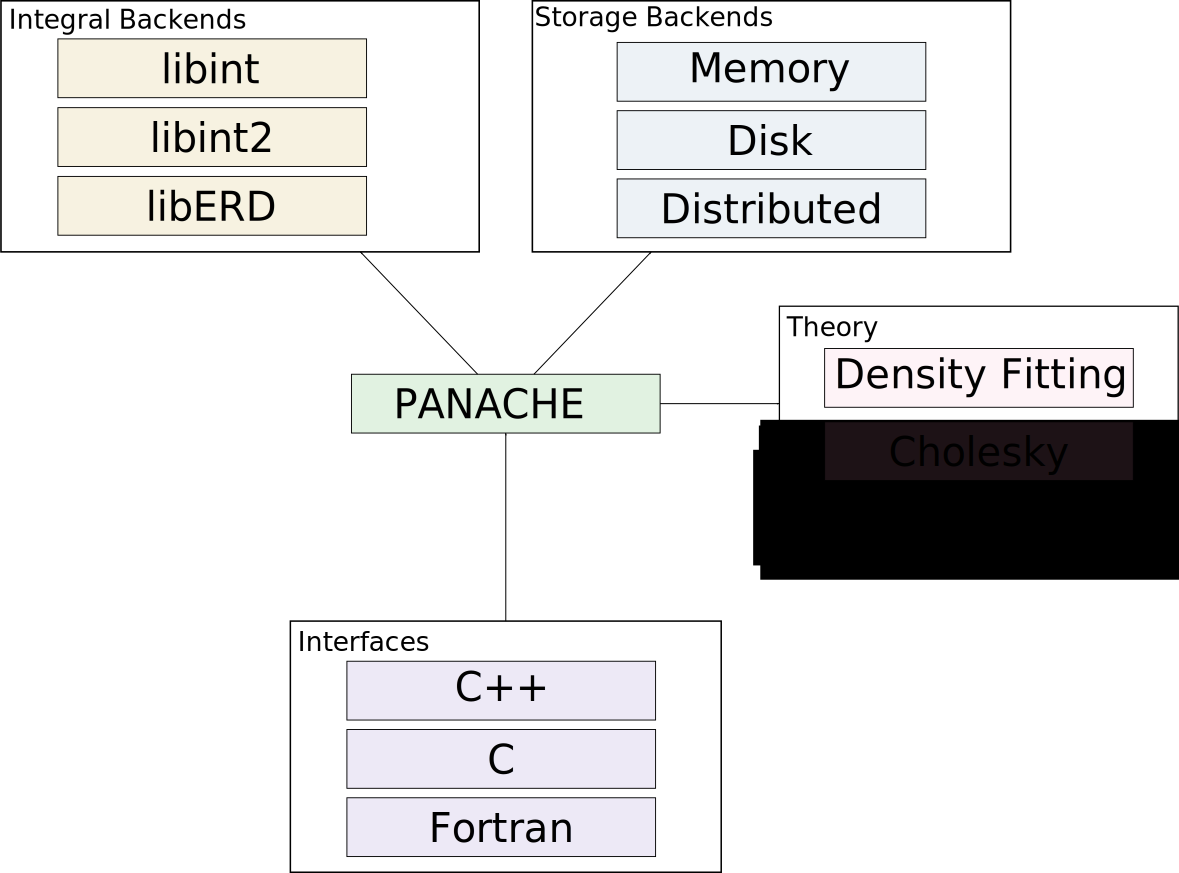
\includegraphics[width=4in]{images/panacheoverview}
\caption{Overview of the structure of the \panache library}
\end{figure}





\subsection{Library Structure}
\label{sec:structure}

The central class of the \panache library is the abstract
\class{ThreeIndexTensor} class (see Figure~\ref{fig:threeindextensor}),
whose main purposes are to provide the common interface to density fitting
and Cholesky decomposition, and to implement common operations (such as
handling of MO coefficient matrices and related transformations). In
general, this class is responsible for the interface for almost all
transformations and other tensor operations, as well as providing a method
for transferring data back to the calling program. Classes derived from
\class{ThreeIndexTensor} (DFTensor and CHTensor for density fitting and
Cholesky decomposition, respectively) are in general only responsible
for generation of the three-index, AO-basis \Qso tensor, where \Qso
is either the $B$ tensor from density fitting or $L$ from Cholesky
decomposition (see Section~\ref{sec:theory})

After the generation, \Qso can be treated the same, independent of
whether it is from density fitting or Cholesky decomposition. This
includes reordering, transformation (to MO basis, etc), storage, and
retrieval by the calling program.  In that sense, it is obvious that the
presented class hierarchy is a natural fit for these theoretical methods.

\begin{figure}
\centering
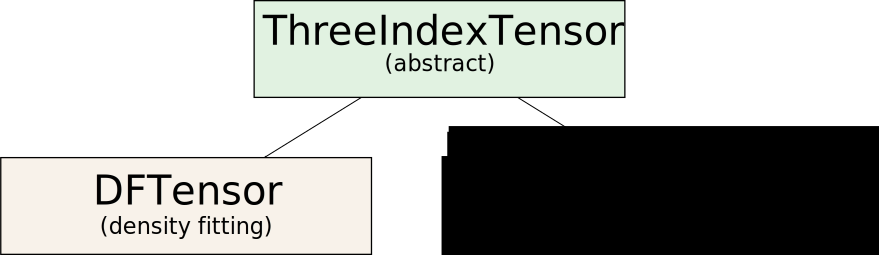
\includegraphics[width=3in]{images/threeindextensor}
\caption{The \class{ThreeIndexTensor} class and its derived classes.}
\label{fig:threeindextensor}
\end{figure}

Actual storage of three-index tensors is implemented
by the \class{StoredQTensor} and its derived classes
(Figure~\ref{fig:storedqtensor}).  Objects of classes derived
from the \class{StoredQTensor} base class are stored in the
\class{ThreeIndexTensor} class.

%
\begin{figure}
\centering
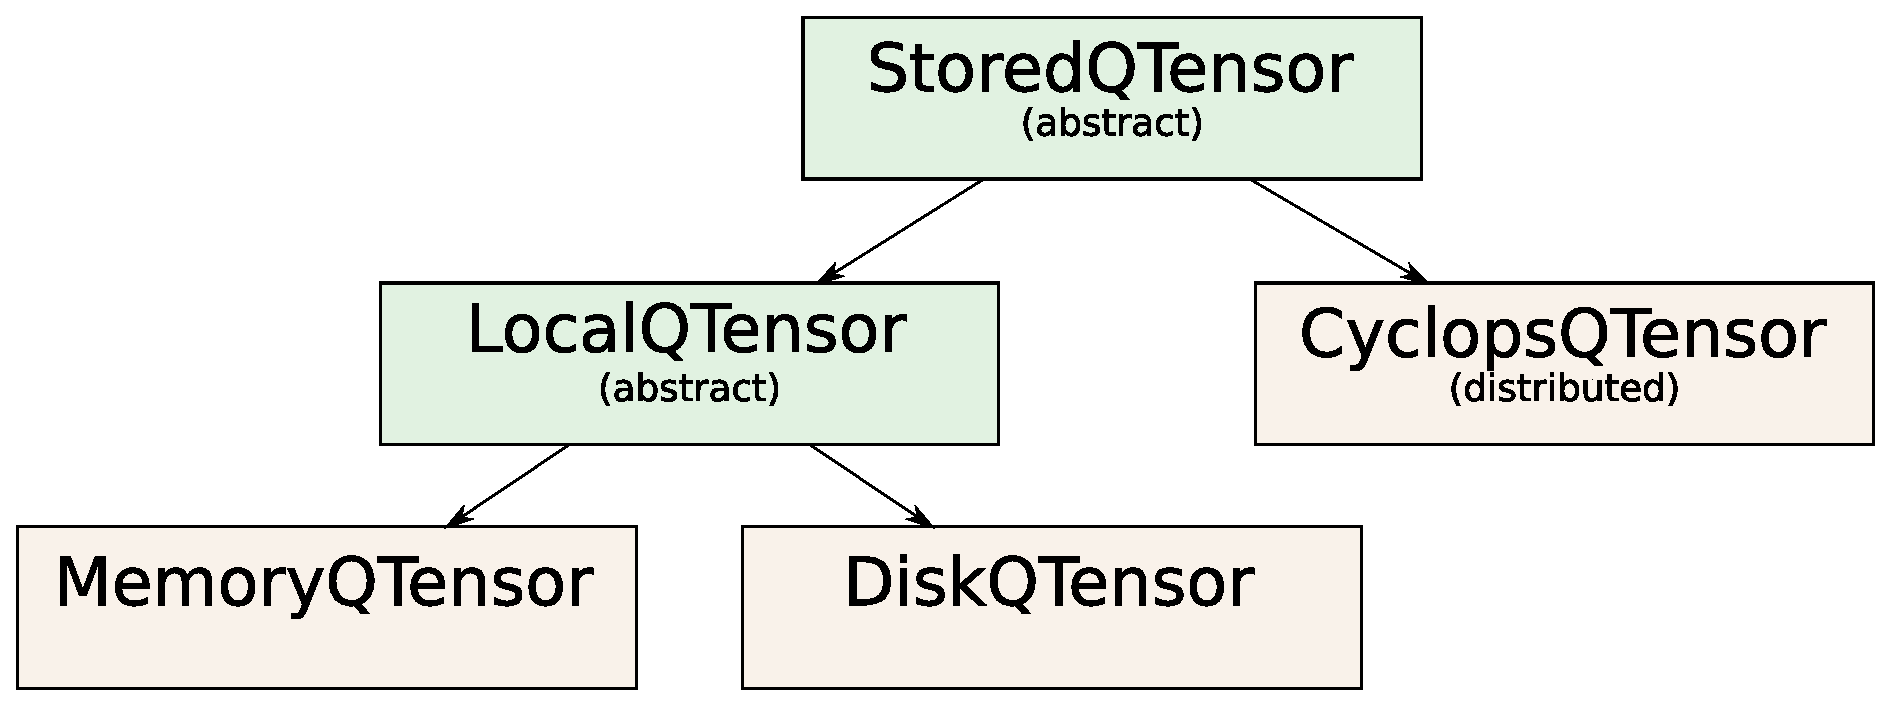
\includegraphics[width=3in]{images/storedqtensor}
\caption{The \class{StoredQTensor} class and its derived classes}
\label{fig:storedqtensor}
\end{figure}
%
Any calculated three-index quantities (from either density fitting
or Cholesky decomposition, and in the AO or MO basis) can be stored
in memory or on disk, with the determination made at runtime. The
tensors may also be kept after the calculation is finished for later
reuse or analysis, and transparently moved from disk to memory. This
is all handled in the \class{LocalQTensor} class and its derived
classes.  For distributed calculation and storage, the Cyclops
Tensor Framework\cite{Solomonik:2012a} (CTF) can be used via the
\class{CyclopsQTensor} class.  It should be noted, however, that because
of the differences in distributed vs single-node storage, aspects of the
generation of \Qso as well as details concerning the MO transformations
are actually contained in the storage classes.

Calculation of two- and three-center ERIs are handled by popular integral
packages; currently, \panache supports libint\cite{LibintLink, Libint1,
Libint2} (both v1 and v2) and libERD\cite{Flocke:2008a} (distributed with
\panache), although adding others is possible. No further linking should
be required for code already utilizing libint.  Extending \panache to
use other integral code is also possible.

Parallelization is achieved primarily via OpenMP (with appropriate
compiler support), although the library is certainly usable when compiled
without it. As mentioned previously, distributed computation of both
density fitting and Cholesky decomposition is experimentally supported
via CTF.


\subsection{Interface}
\label{sec:interface}

The interface to \panache includes passing in the required information
(such as the basis set and density fitting basis set, or the Cholesky
decomposition cutoff), transformation to specified the MO basis (or
subsets such as occupied-occupied), specification of storage class (disk,
memory), and retrieval of the required three-index tensors for use by
the calling code.

Because of the diversity of existing computational chemistry software,
the interface to \panache was made as flexible and as extensible as
possible. The core interface to the library is its C++ interface, however
C and Fortran bindings are included. The Fortran interface is written in
Fortran 2003, allowing for transparent conversion between C and Fortran
data types and name-mangling conventions (that is, uppercase function
names and trailing underscores). It should be noted that although the
Fortran interface is written Fortran 2003, software written in older
Fortran standards will still be able to function with \panache. In
addition, due to the relatively straightforward C interface, it should
be possible to use it with any language that supports C bindings, such
as Python.

One major issue with interfacing with existing codes is the difference
in ordering with a particular Gaussian (spherical or cartesian)
shell. To help with this \panache includes the ability to reorder its
integrals. When possible, this is done efficiently by only reordering
the MO coefficients, rather than any generated three-index tensors. This
reordering capability currently supports PSI4 (default), GAMESS, and
Dalton ordering, but is easily extended if needed. Internally, \panache
uses the same ordering as that used in Psi4.

Lastly, for existing software where implementing parsing and storage of
the auxiliary basis set needed for density fitting may be difficult,
the library supports constructing the auxiliary basis from a given
Gaussian-formatted basis set file and information describing the molecule.

To test the library, implementations of calculation of MP2 correlation
energy\cite{Werner:2003a} were successfully developed for the
PSI4\cite{Turney:2012a}, GAMESS\cite{Gamessbook, Schmidt:1993a}, and
DALTON\cite{DaltonLink, Dalton} packages. THe MP2 correlation energy was
successfully calculated using both both density fitting and Cholesky
decomposition utilizing the geometry, basis set, and MO coefficients
passed from the calling code.

Details on how the interfaces are used can be found in the \panache
documentation.


\subsection{Conclusion and Future work}
\label{sec:plans}

The \panache library provides a modular, efficient approach to calculation
of approximate electron repulsion integrals via density fitting and
Cholesky decomposition.  It is designed to be flexible and able to be
incorporated into existing computational chemistry software via C++, C,
and Fortran bindings.

Parallelization is achieved via OpenMP; support for distributed
computational is currently experimental and is planned to be expanded
in the future to other tensor libraries.


\section{Availability and Documentation}
\label{sec:availability}

\edit{Correct?}
The \panache library is available at GitHub at \edit{address} and is licensed under
the GNU General Public License (GPL).

Extensive bulding and usage documentation, as well as code documentation,
is available at http://www.psicode.org/panache.php.


\section{Acknowledgements}
\label{sec:ack}
This research was funded by the U.S. National Science Foundation (Grant No. ACI-1147794)


%\bibliographystyle{achemso}
\bibliography{references}

\end{document}
